\chapter{State of the Art} \label{chapter:sota}

\section{Positioning systems and indoor navigation} \label{2:indoor_navigation}

    Nowadays, location tracking and outdoor navigation are commonplace, thanks to \gls{gps} technology. In order to determine the location of a mobile device, the distance between the device and several (i.e. at least three) satellites is measured, in a process called \textbf{trilateration} (fig. \ref{2:fig:gps_trilateration}) \cite{gis2021trilateration}. For additional accuracy, a similar procedure (sometimes called \textbf{triangulation}) is done using the distance to nearby GSM (cell) towers \cite{radiojitter2018triangulation}.
    
    \begin{figure}[ht]
        \centering
             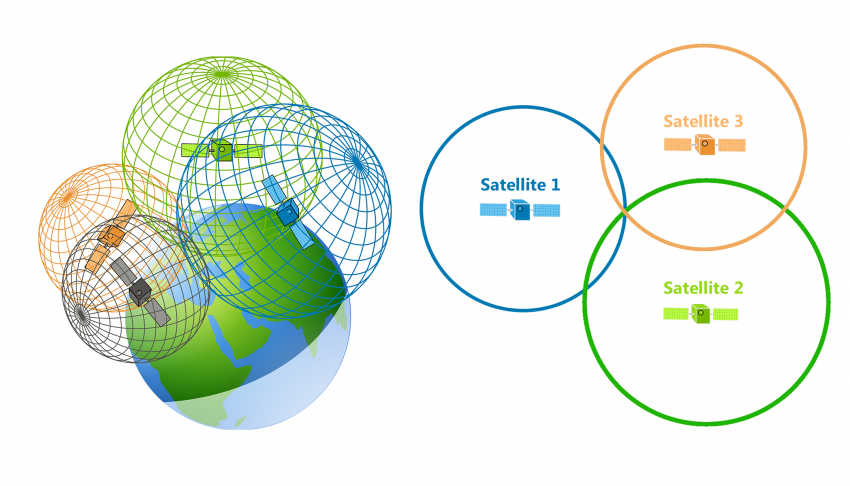
\includegraphics[width=\textwidth]{figures/gps.png}
        \caption{\gls{gps} trilateration}
        \label{2:fig:gps_trilateration}
    \end{figure}
    
    The \gls{gps} performance standard \cite{gps2008performance} promises an accuracy of <7.8m 95\% of the time, with "well designed \gls{gps} receivers" achieving a horizontal accuracy of <3m. Several factors can weaken \gls{gps} signals, including mountains and thicker walls of a building. Consequently, \gls{gps} alone cannot be used in the context of indoor navigation since, in order to distinguish between different rooms, an accuracy of at least 2m would be necessary. Furthermore, vertical accuracy is approximately two times worse than horizontal accuracy, meaning that distinguishing between floors in multi-story buildings is nearly impossible using only a \gls{gps} signal. 
    
    Due to the issues underlined above, indoor navigation is a complex computing problem which requires a special network of devices used to locate a person or an object in environments where \gls{gps} technology fails, called an \acrlong{ips} (\acrshort{ips}). Any wireless signal (such as \textbf{Wi-Fi}, \textbf{Bluetooth}, \textbf{\acrshort{rfid}} or \textbf{\acrshort{ir}}) can be used for locating. Combining multiple different signals can lead to greater accuracy - as is the premise of the AirDocs project, described more in appendix \ref{a:airdocs}. 
    Furthermore, non-radio technologies can also be used for indoor positioning. \textbf{Magnetic positioning} measures local variations in the Earth's magnetic field caused by the amount of iron inside buildings. As seen from the system described by Guido de Angelis Et Al. \cite{de2014indoor}, this method can achieve an accuracy of <10cm but requires costly sensors and is not feasible in the context of a mobile device. \textbf{Inertial positioning} can use the accelerometer/pedometer of a phone to track the steps of the users and approximate the distance travelled with an accuracy of <0.5m, as described by Qiu and Mutka \cite{qiu2017self}. Finally, camera-enabled devices can use \textbf{positioning based on visual markers}, which is the technology used by Google Maps AR Navigation\footnote{\url{https://www.cnbc.com/2019/08/08/google-maps-ar-directions-released-for-iphones-and-android.html}}.


\section{Maps APIs} \label{2:maps_apis}

    The most popular Maps APIs are Google Maps\footnote{\url{https://developers.google.com/maps/documentation}}, Bing Maps\footnote{\url{https://www.bingmapsportal.com/}} and Apple Maps\footnote{\url{https://developer.apple.com/maps/}}. Out of these, Apple Maps only works on iOS and, therefore, would be a poor choice for our cross-platform application. None of the APIs provides support for navigating inside custom buildings - indoor navigation is only allowed for specific public buildings like malls and airports.
    
    According to Tirena Dingeldein \cite{dingeldein2019bingvsgoogle}, Bing offers higher image quality and a friendlier API, but Google Maps has better navigation algorithms and a better mobile experience. Furthermore, Google Maps is highly compatible with the Google-centric development environment that \gls{app} uses (see section \ref{1:faculty_app}).
    
    Bryan Boyd Et Al. \cite{boydcampus} from Texas A\&M University describe a web-based navigation system based on the Google Maps API. The system does not include indoor navigation, but it accounts for different modes of transportation such as walking, driving or taking the bus. These modes are achieved through a layered roadmap (fig. \ref{2:fig:roadmap_layering}), in which the roadmap is represented through a graph, where vertices are \acrshort{poi}s and edges are roads or "transition edges" (for changing between transportation modes).
    
    \begin{figure}[ht]
        \centering
             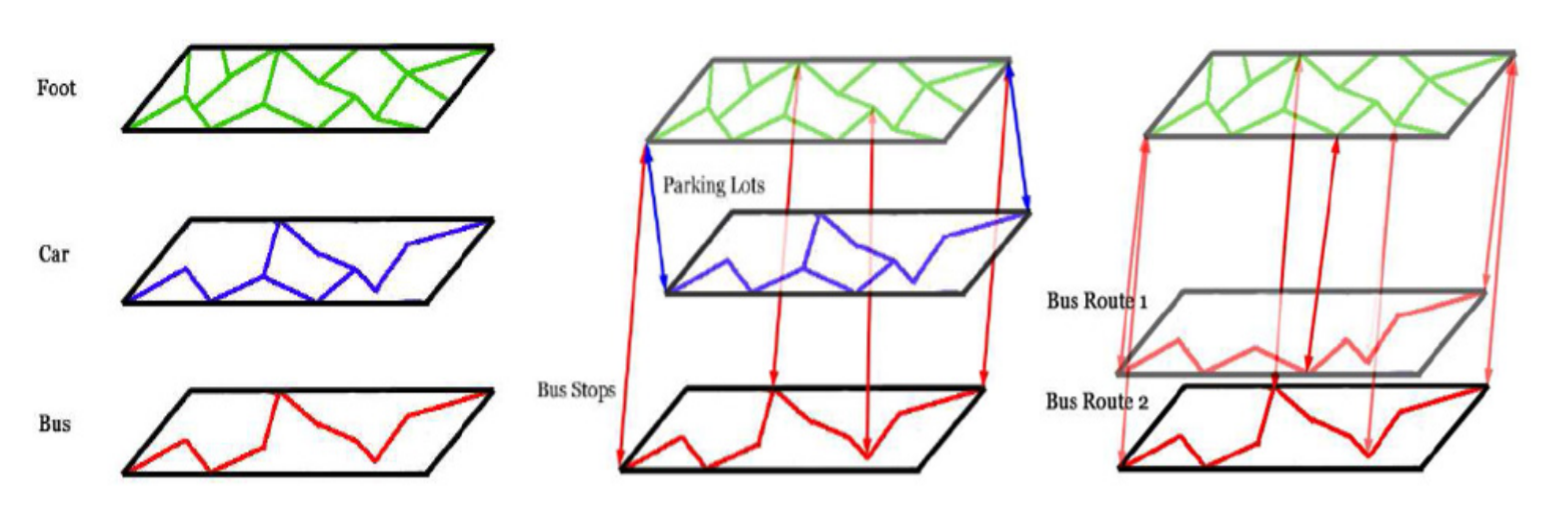
\includegraphics[width=\textwidth]{figures/roadmap_layering.png}
        \caption{Roadmap layering, transition edges and sub-layering}
        \label{2:fig:roadmap_layering}
    \end{figure}
    
\section{AR indoor positioning} \label{2:ar_indoor_positioning}
        
    As previously discussed in section \ref{2:indoor_navigation}, accurate localization inside a building is difficult to achieve with only GPS, without additional sensors or hardware such as Bluetooth beacons or WiFi signal triangulation. A different approach to indoor navigation would be to use an AR-based solution to find the user’s location (through a VPS, or Visual Positioning System) and guide them to their destination.
    
    AR-based navigation is not a new concept, but it has only recently become more reliable and started to find its way into the consumer market, most notably through Google Maps’ Live View, first launched in 2019\cite{ranieri2020liveview}.
    
        \subsection{Visual Positioning System} \label{2:visual_positioning_system}
        
        While GPS (Global Positioning System) is a space-based radio-navigation system using signal from satellites, VPS (Visual Positioning System) aims to achieve positioning using an approach that is more similar to human behaviour. In the same way we look around to understand the world and our location, VPS means looking at an image of the user’s surroundings and matching against its database of locations (“visual markers”) to guess where the user is currently located.
        
        Google Maps Live View’s VPS works by asking the user to move their phone around them to capture the surroundings, and then comparing the camera data with its extensive Street View database in order to determine the user’s location. This mostly works outdoors (and works better in daylight), but Google has slowly been expanding this functionality to some indoor spaces such as airports\cite{glasgow2021mapai}  and some transit stations in Japan\cite{gmaps2021japan}. One of the biggest challenges in using VPS in public spaces is the crowd - in densely circulated areas, it is unlikely that the user would be able to get a clear view of the static surroundings without a lot of people in the frame, which then have to be “erased”\cite{senzer2021magiceraser} using machine learning in order for the VPS to work its magic.
        
        Unfortunately, the APIs used for AR navigation in Google Maps are not (yet) public. However, similar technologies by Apple - AR location markers\footnote{\url{https://developer.apple.com/documentation/arkit/content_anchors/tracking_geographic_locations_in_ar}} - are currently available within ARKit, the AR framework for iOS devices.

        \subsection{Technologies} \label{2:ar_technologies}
        
        There are currently two main platforms used for development of AR navigation solutions on mobile devices: ARKit for iOS and ARCore for Android. These development environments are responsible for translating information captured by device sensors such as the camera and gyroscope in order to draw virtual objects on the screen so that they appear to reside in the real world.
        
            \subsubsection{ARKit} \label{2:arkit}
            
            According to Mobidev\cite{makarov2021arnavigation}, ARKit is generally regarded as the more powerful of these two powerful mobile AR platforms, thanks to being backed up by more reliable hardware and software. Apple has full control over the production and design of its iPhone and iPad hardware as well as the OS software, whereas there is a great deal of hardware and software diversity between one Android phone to another due to the large number of different manufacturers. Because of this, ARKit’s performance is better optimised.
            
            One of the key features that puts iPhones above Android devices in the AR arena is the LiDAR sensor. This hardware can make AR navigation easier due to its depth sensing capabilities, and can reduce the need for specialised mapping hardware such as a 3D camera.
            
            \subsubsection{ARCore} \label{2:arcore}

            Although ARCore may not be as powerful as ARKit due to current hardware limitations and inconsistencies, it is still a very valuable platform that cannot be overlooked. Based on a survey with 200+ respondents\cite{alexandru2020acsupbmobile}, roughly 80\% of students in the Faculty of Automatic Control and Computers own Android devices. Due to this majority, we cannot focus solely on an iOS-only solution, and need to find a middle ground that can work on most mobile devices.
            
            A major advantage in focusing on ARCore is that, while ARKit only works for iOS devices, ARCore is compatible with both Android and iOS devices\footnote{\url{https://developers.google.com/ar/devices}}. This makes it a good medium through which to achieve a cross-platform solution, even though it doesn’t (yet) offer out-of-the-box capabilities for VPS.
            
            \subsubsection{Other approaches} \label{2:other_ar_approaches}
            
            It is worth mentioning that aside from the “canonical” AR platforms, there are custom solutions (generally built on top of the above) that promise to provide AR frameworks with various features.
            
            One such solution is used in Matthew Hallberg's demo\footnote{\url{https://www.youtube.com/watch?v=VOMysKbDNxk}} - Placenote\footnote{\url{https://placenote.com/}}  offers an AR SDK that allows users to scan their surroundings to generate a 3D model, and can be very useful for mapping an indoor space for the purpose of navigation.

            Ennio Pirolo from Ambiens VR describes a different approach\footnote{\url{https://www.youtube.com/watch?v=PQmMiB9BRYU}}, which uses specialized ArchViz (architectural rendering) tools to create the map of the indoor space into Unity, to then use for the navigation. Specifically, it uses Revit and some special ArchViz packages for syncing Unity and Revit (AT+Sync for Unity\footnote{\url{https://assetstore.unity.com/packages/tools/integration/at-sync-v2-synchronize-from-revit-182941}} and Revit\footnote{\url{https://apps.autodesk.com/RVT/en/Detail/Index?id=4892322793396128687}}, AT+Explore\footnote{\url{https://assetstore.unity.com/packages/tools/visual-scripting/at-explore-interactive-archviz-137202}}).
            
            Yet another solution\footnote{\url{https://www.youtube.com/watch?v=F5wqfYKVbv0}}, from Joshua Drewlow, uses Vuforia Engine with area targets\footnote{\url{https://library.vuforia.com/features/environments/area-targets.html}} - an environment tracking feature that enables you to track and augment areas and spaces, based on ARKit’s location markers. This only works with an ARKit-enabled iOS device with a LIDAR sensor, in addition to a 3D camera (Matterport™ Pro2 3D) and special scanners (avVis M6 and VLX, Leica BLK360 and RTC360).

\section{Existing navigation tools for our campus} \label{2:existing_tools}

    As described in the previous paper\cite{alexandru2020acsupbmobile}, there have been several attempts at providing campus navigation for \acrlong{upb}. In April 2019, a group of students attempted to create an Android app that provides indoor navigation instructions\footnote{\url{https://github.com/IrinaM09/UPB}}, as a group project for their software engineering class. The project, however, remained in the state of a simple proof of concept (fig. \ref{2:fig:upb_campus_unpublished}), since the lack of existing digital data of the room layout in the campus buildings meant that they had to manually write the information in the form of a graph in a \gls{json}\footnote{\url{https://github.com/IrinaM09/UPB/blob/master/app/src/main/res/raw/nodes.json}} file. This process proved to be extremely tedious.
    
    \begin{figure}[!ht]
        \centering
        \begin{minipage}[b]{\textwidth}
            \captionsetup{justification=centering}
             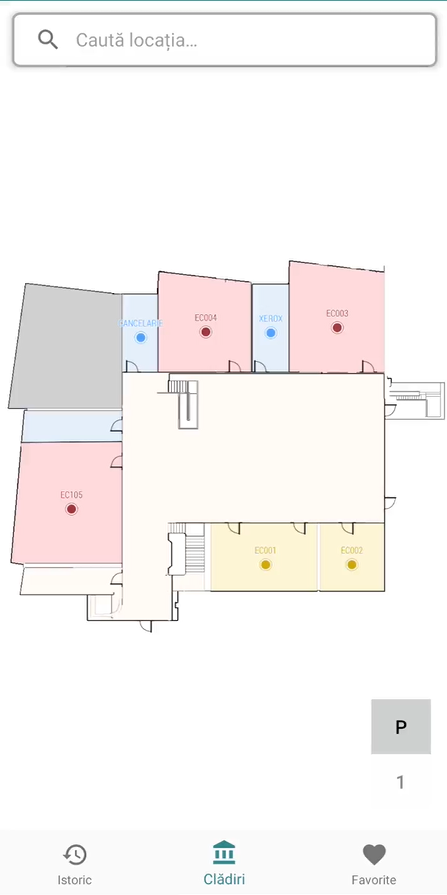
\includegraphics[width=0.49\textwidth]{figures/navigation_apps/upb_campus_unpublished1.png}
             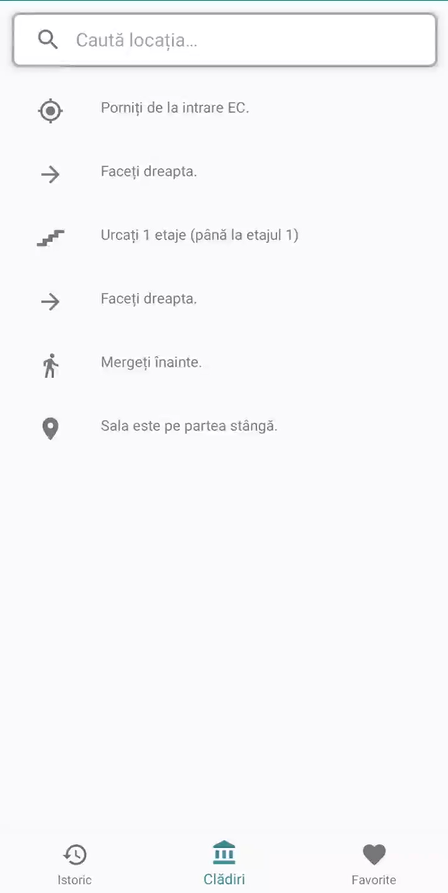
\includegraphics[width=0.49\textwidth]{figures/navigation_apps/upb_campus_unpublished2.png}
            \caption{Unpublished \acrshort{upb} campus map application}
            \label{2:fig:upb_campus_unpublished}
        \end{minipage}
    \end{figure}
    
    \newpage
    
    Roughly a year later and entirely separately, a student from the Faculty of Engineering in Foreign Languages\footnote{\url{http://ing.pub.ro/en/}} within \acrshort{upb}, with a passion for programming,  wrote a paper\cite{scurtu2020upb} for the \acrshort{upb} Students Scientific Communications Session. Consequently, they won a prize and published a campus map mobile application for both iOS and Android devices (fig. \ref{2:fig:upb_campus_published}), using the Apple Maps and the Google Maps APIs, respectively (see section \ref{2:maps_apis}). It later became the official UPB app and gained many more features and a new look (fig. \ref{2:fig:upb_campus_new_published}).
    
    \begin{figure}[!ht]
        \centering
        \begin{minipage}[b]{0.49\textwidth}
            \captionsetup{justification=centering}
             
\includegraphics[width=0.49\textwidth]{figures/navigation_apps/upb_campus_published1.png}
             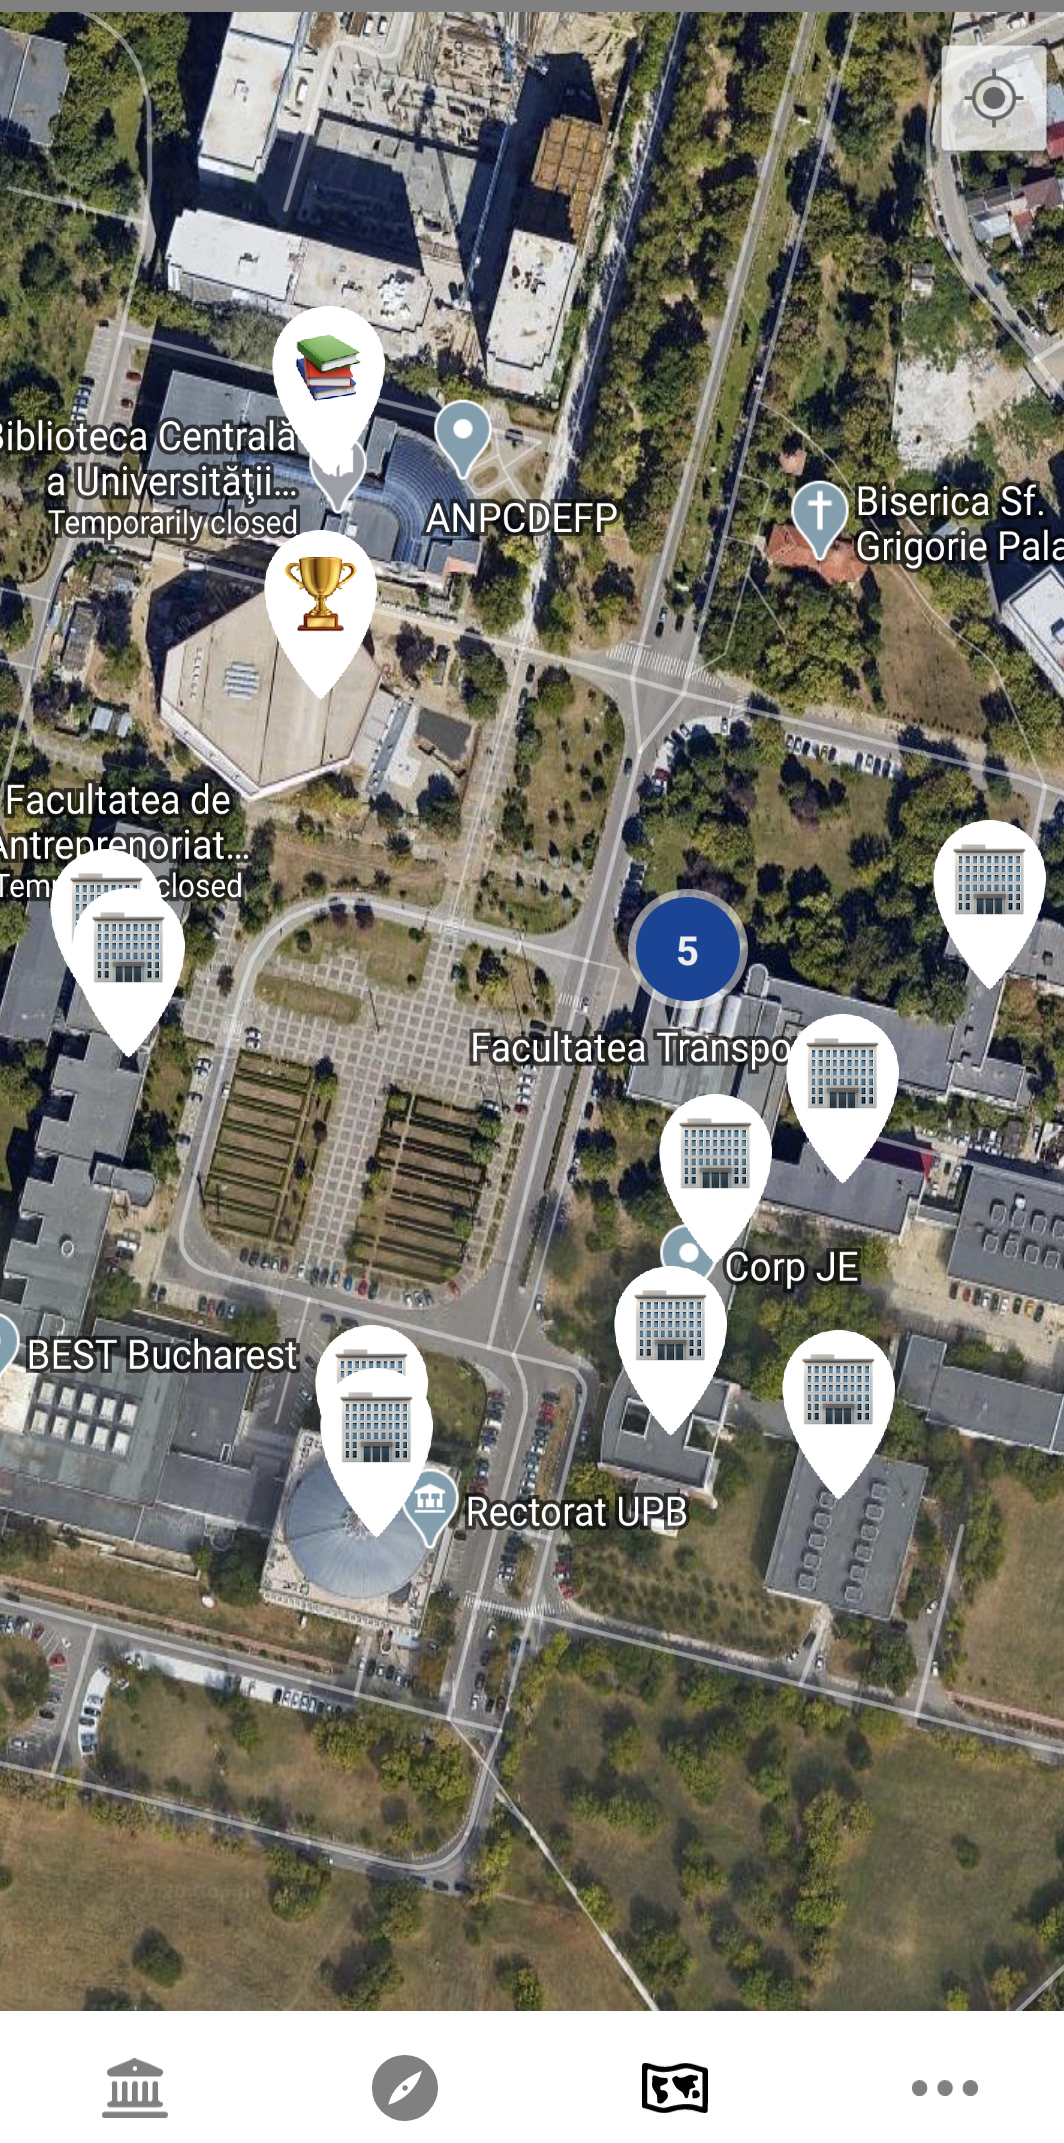
\includegraphics[width=0.49\textwidth]{figures/navigation_apps/upb_campus_published2.png}
            \caption{Published \acrshort{upb} campus map application (2020)}
            \label{2:fig:upb_campus_published}
        \end{minipage}
        \hfill
        \begin{minipage}[b]{0.49\textwidth}
            \captionsetup{justification=centering}
             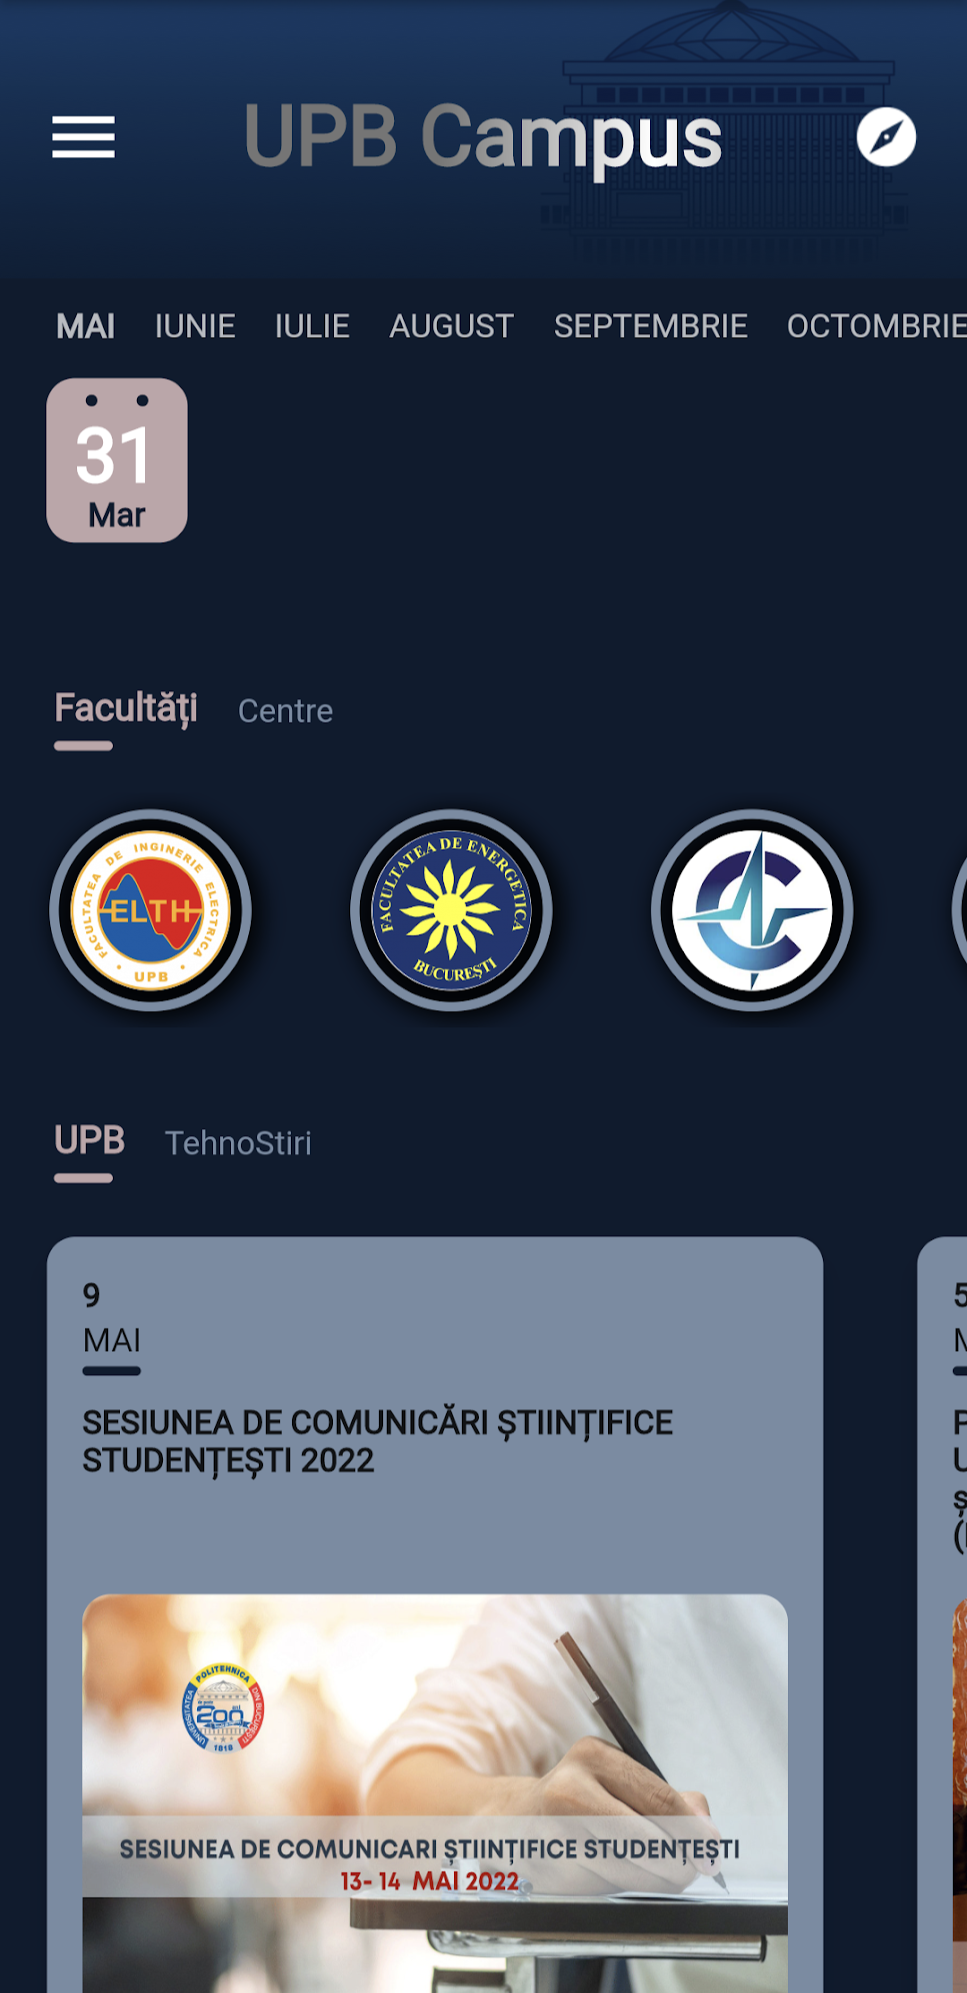
\includegraphics[width=0.49\textwidth]{figures/navigation_apps/upb_campus_new_published1.png}
             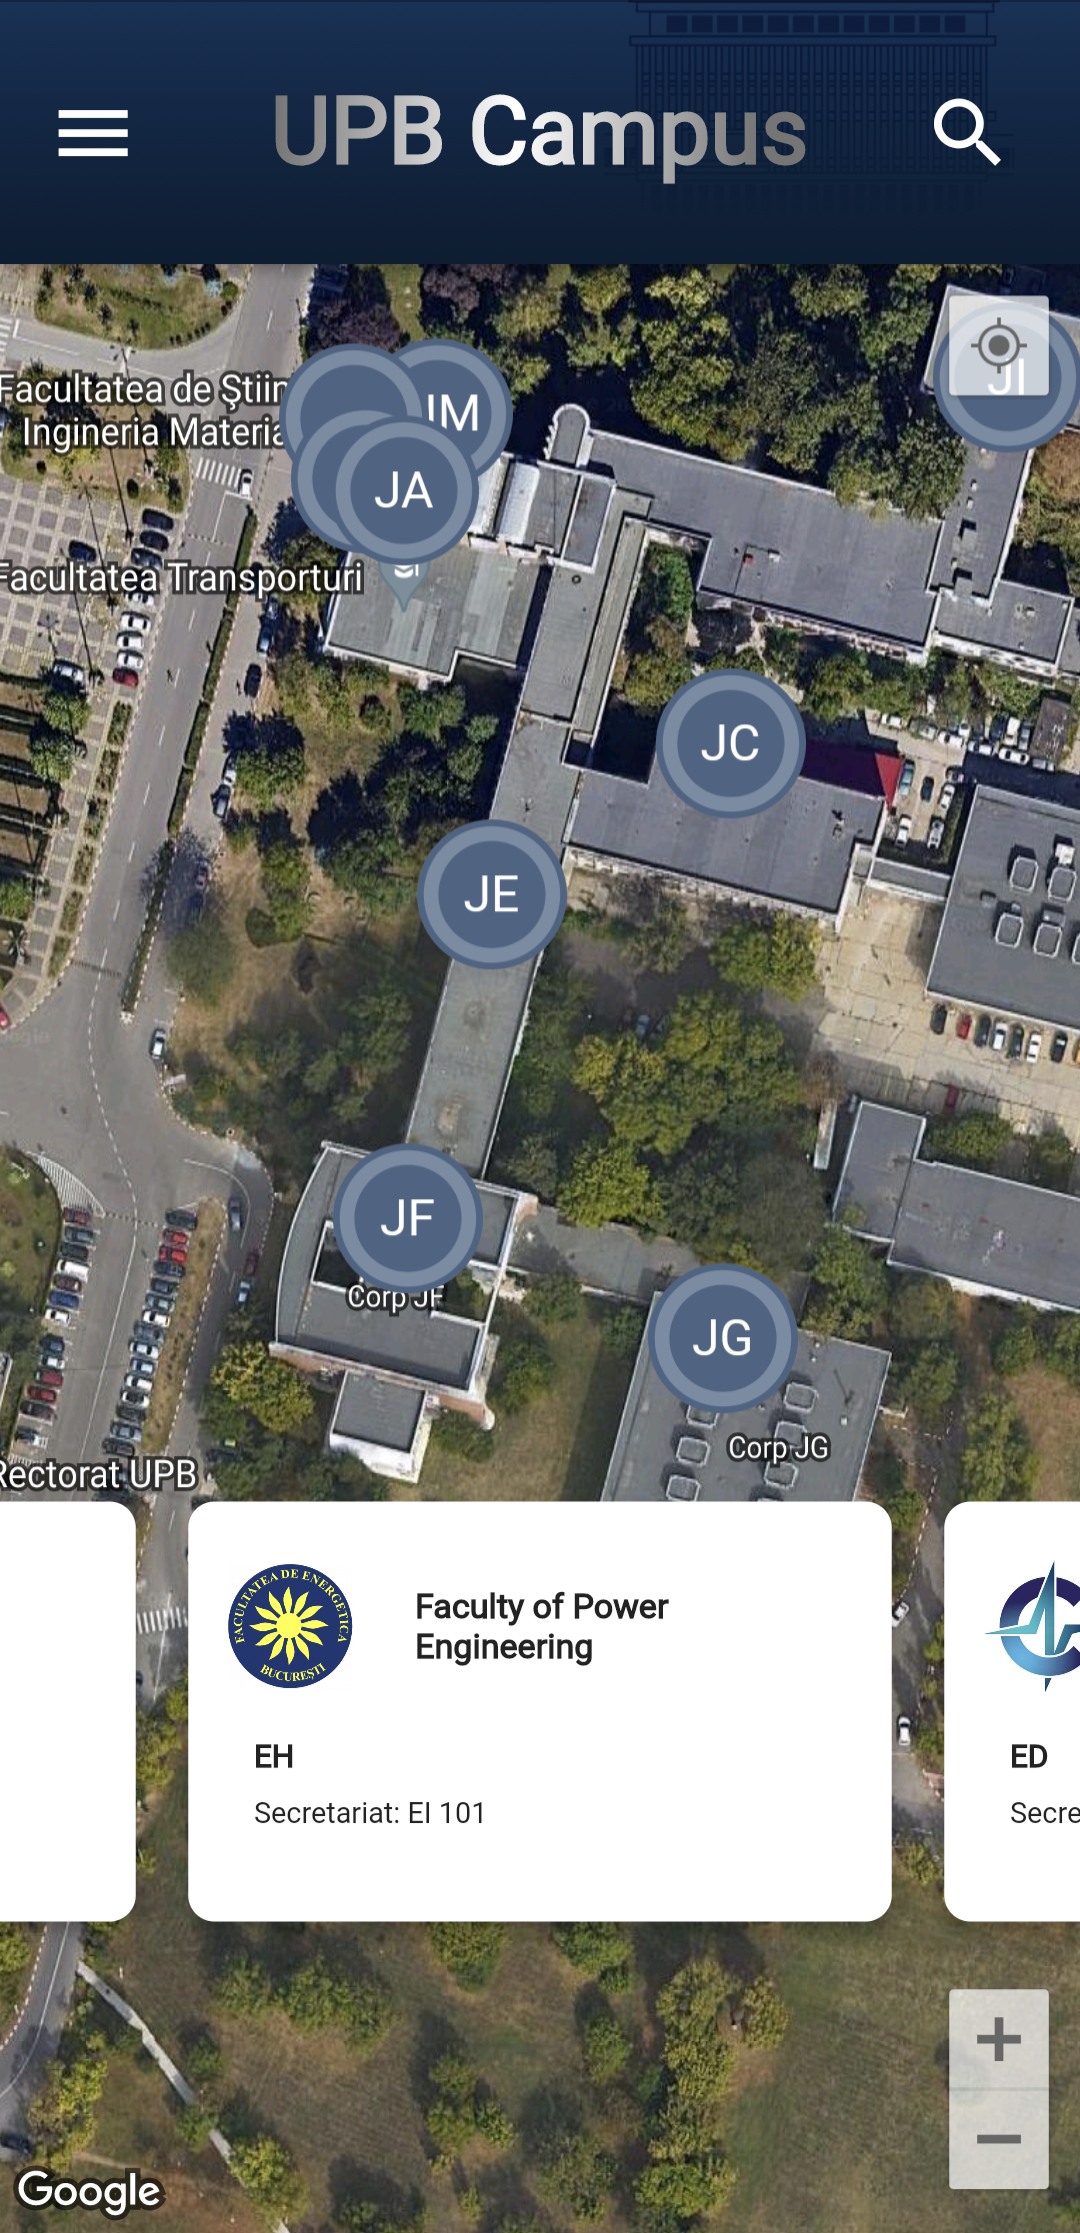
\includegraphics[width=0.49\textwidth]{figures/navigation_apps/upb_campus_new_published2.png}
            \caption{Published \acrshort{upb} campus map application (2022)}
            \label{2:fig:upb_campus_new_published}
        \end{minipage}
    \end{figure}
    
    ~
    
    While admittedly not a navigation tool per se, another project that deserves a mention in this section is 3DUPB\footnote{\url{http://3d.pub.ro/}}. It is a computer graphics summer school involving a project that revolves around a 3D model of the \acrlong{acs} (fig. \ref{2:fig:3dupb_outside}, \ref{2:fig:3dupb_inside}).
    
    \begin{figure}[!ht]
        \centering
        \begin{minipage}[b]{0.49\textwidth}
            \captionsetup{justification=centering}
             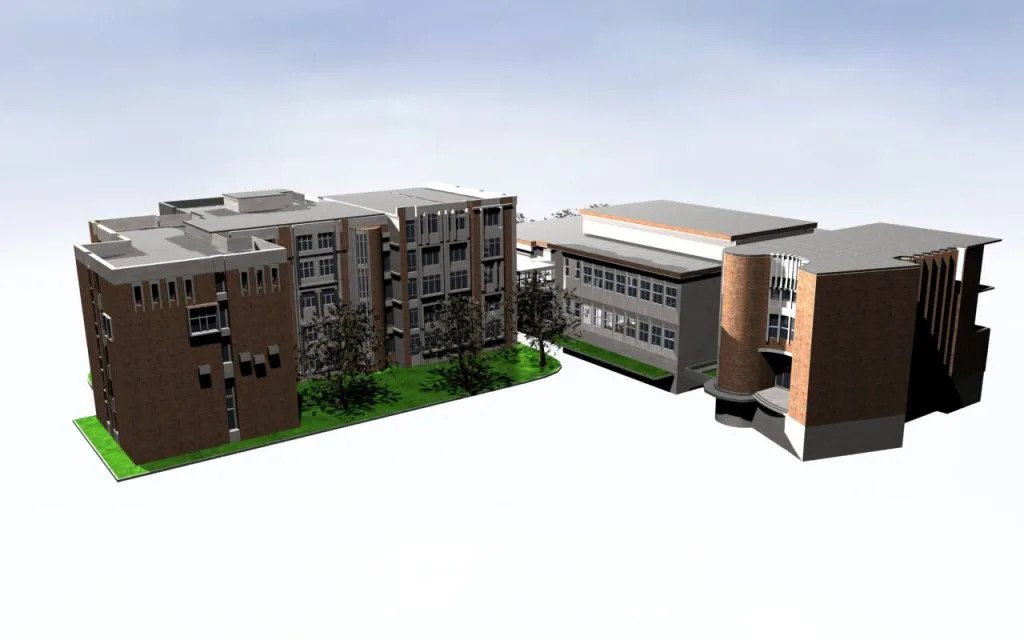
\includegraphics[width=\textwidth]{figures/navigation_apps/3dupb_outside.jpg}
            \caption{3D model of the outside of \acrshort{acs} (from 3DUPB)}
            \label{2:fig:3dupb_outside}
        \end{minipage}
        \hfill
        \begin{minipage}[b]{0.49\textwidth}
            \captionsetup{justification=centering}
             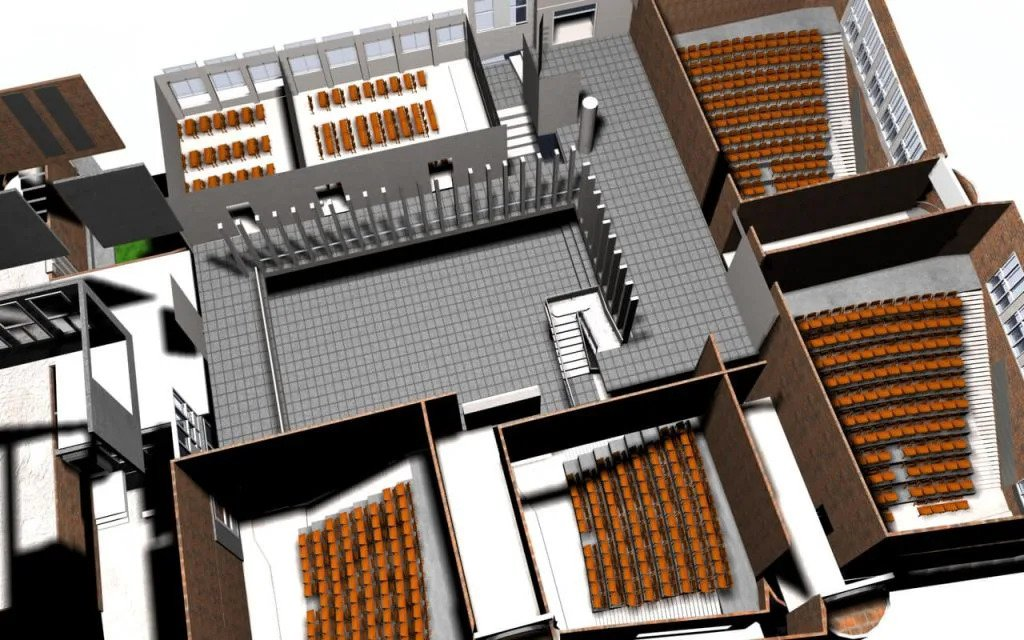
\includegraphics[width=\textwidth]{figures/navigation_apps/3dupb_inside.jpg}
            \caption{3D model of the inside of \acrshort{acs} (from 3DPUB)}
            \label{2:fig:3dupb_inside}
        \end{minipage}
    \end{figure}
    
    Given the 3D models, a 3D campus navigation system would be possible. However, several challenges are involved with such a system. The most crucial challenge is that rendering a complex 3D model consumes a lot of time and resources and may be infeasible for a mobile device. Additionally, any change in the structure of the building would require remodelling.
    
    In 2009, Jing Wang and Zhi Lin \cite{wang2009general} from the Asian Institute of Technology proposed a web-based 3D Campus Navigation System. In a similar fashion to the navigation system described in section \ref{2:maps_apis}, this campus navigator uses a graph to represent buildings (vertices) and roads (edges). It is described as being made up of four modules: the spatial environment module, the nodal graph module, the animation module and the behaviour module. The spatial environment module creates 3D models of each campus building in a spatial environment. The nodal graph module calculates the shortest path between the nodes defined based on the spatial environment (where each building is assigned a node near its main entrance). The animation module deals with displaying the user's 3D avatar moving through the map and showing a top-down view in the form of a mini-map. Finally, the behaviour module is responsible for user interactions.

%\section{Other university apps} \label{2:uni_apps}

%TODO maybe